\chapter{Materiais e Métodos}

\section{Climatologia de Ventos}
\label{sec:windClimatology}

\hspace{6mm} Serão utilizados dois tipos de dados (Tabela~\ref{tab:dataset}) da componente
zonal e meridional do vento a 10 metros de altura da superfície: dados de reanálise e
dados \textit{in situ}. Os dados de reanálises serão extraídos do \textit{Climate
Forecast System Reanalysis} (CFSR), para os meses de Dezembro, Janeiro, Fevereiro e
Março, compreendidos entre 1979 e 2010. Quanto aos dados \textit{in situ}
serão extraídos do Programa Nacional de Boias (PNBOIA) das bóias 157597 (Santa Catarina)
e 69009 (Cabo Frio). Mais informações sobre os conjuntos de reanálise são descritos em
\cite{Saha2010} e \cite{Berrisford2011}.

% Inicialmente serão extraídos dados da componente zonal e meridional
% do vento a 10 metros de altura da superfície, a fim de comparar com dados
% \textit{in situ}, para determinação de qual conjunto de dados melhor representa
% o cenário de ventos da PCSE. Em seguida, serão extraídos os mesmos dados de vento
% para os meses de Janeiro, Fevereiro e Março entre 1979 e 2010. Estes dados serão
% então utilizados para elaboração da climatologia de ventos da região. Os conjuntos
% de dados a serem utilizados estão apresentados de forma mais detalhada na
% Tabela~\ref{tab:dataset}.
\bigskip
\begin{center}
\begin{tablehere}
\caption{Conjunto de dados que serão utilizados.}
\label{tab:dataset}
\begin{tabular}{|c|c|c|}

\hline
\textbf{Conjunto de Dados}                   & \textbf{Tipo}    & \textbf{Região}      \\ \hline
CFSR    & Reanálise        & -20$^o$/-30$^o$; -40$^o$/-50$^o$ \\ \hline
PNBOIA - 157597 & \textit{in situ} & -28.51$^o$; -47.39$^o$     \\ \hline
PNBOIA - 69009  & \textit{in situ} & -22.98$^o$; -42.10$^o$     \\ \hline
\end{tabular}
\end{tablehere}
\bigskip
\end{center}

\section{Modelagem Numérica da Circulação}
\label{sec:numericalModelling}

% roteiro:
% apresentar secom
% apresentar falar de algumas coisas: grade, condições de contorno (fechada: no slip boundary, aberta: elevação/maré?)
% falar dos dados que serão implementados: batimetria, vento, TS, maré e outros

\hspace{5mm} Para analisar a circulação na região de interesse, será implementado o modelo \textit{Stevens
Estuarine and Coastal Ocean Model} (sECOM), incluindo as forçantes vento, maré e gradiente de densidade,
sendo este modelo um variante do \textit{Princeton Ocean Model} (POM) \citep{Blumberg1987}.

\hspace{5mm} Este é um modelo numérico de circulação costeira e estuarina, tridimensional, que utiliza equações primitivas empregando
grades C de Arakawa em conjunto com o sistema de coordenadas $\sigma$ na vertical, no processo de discretização.
Dentre os módulos existentes no sECOM, neste trabalho será utilizado somente o Módulo Hidrodinâmico,
descrito no item a seguir.


\subsection{Módulo Hidrodinâmico}
\label{sub:hydrodynamicModule}

\hspace{5mm} As equações deste módulo descrevem os campos de velocidade, elevação da superfície livre,
temperatura e salinidade. Para isso, utiliza duas aproximações:
\begin{enumerate*}[label=(\alph*)]
  \item aproximação hidrostática, que considera o equilíbrio entre o peso do fluido e a força de gradiente de
  pressão na vertical e
  \item aproximação de Boussinesq, ignorando as variações de densidade, exceto quando são multiplicadas pela
  gravidade.
\end{enumerate*}
O conjunto de equações resolvido pelo modelo envolve a conversação de massa, momento, calor e
sal, em função da velocidade, temperatura ($T$) e salinidade ($S$) \citep{Harbor1999}.

\hspace{5mm} Além das equações citadas, o módulo hidrodinâmico parametriza a turbulência baseado no trabalho de 
\citep{mellor1974hierarchy}, onde os coeficientes de difusão turbulenta são obtidos através do esquema de fechamento turbulento de segunda ordem \cite{mellor1982development}.

\subsection{Domínio}
\label{sub:domain}

% Grade, condições de contorno conhecidas (Reid e Bodine [1968], aberta. no slip boundary condition, fechada)
\hspace{5mm} A grade numérica que será utilizada neste trabalho (Figura~\ref{fig:areaestudo}) foi elaborada
em \cite{pereira2007numerical} e adaptada pelo Laboratório de Hidrodinâmica Costeira (LHiCo), para remoção
das células secas. Trata-se de uma grade ortogonal e curvilínea, com 110 pontos na direção $x$, há
uma resolução horizontal variando de 0.5 km a 5 km nesta direção Na direção $y$, 137 pontos,
com uma resolução horizontal variando de 0.5 km, na parte mais central, a 35 km nas regiões com profundidade
superiores a 2100 m. A resolução vertical é de 37 níveis sigma, sendo $\sigma = 0$ na superfície e $\sigma = -1$
no fundo.

\hspace{5mm} Nos experimentos numéricos será considerada a condição de livre escorregamento
nos contorno laterais fechados, ou seja, próximos a costa. Nos contornos abertos será implementada
a condição radiativa, elaborada por \citep{reid1968numerical}, onde o contorno será forçado
pela elevação da superfície livre do mar influenciada pela maré.


\begin{figure}[!h]
    \centering
    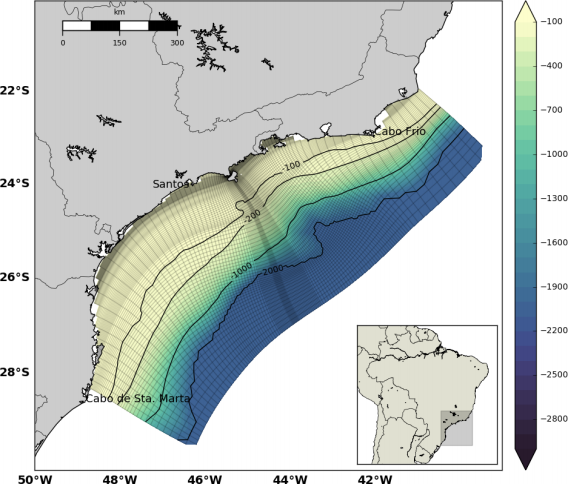
\includegraphics[width=0.7\textwidth]{figuras/grade.png}
\caption[Plataforma Continental Sudeste]{Localização da Plataforma Continental Sudeste, com dados batimétricos fornecidos
pelo Laboratório de Hidrodinâmica Costeira (LHiCo) e grade numérica adaptada de \cite{pereira2007numerical}.}
    \label{fig:areaestudo}
\end{figure}

% condições iniciais está faltando

\subsection{Forçantes}
\label{sub:forcing}


% \hspace{5mm} Batimetria

\hspace{5mm} Os dados de vento serão extraídos do CSFv2, para o meses de Dezembro de 2013 a Março de 2014, que 
serão interpolados espacialmente para a resolução da grade numérica utilizada, preservando-se a resolução
temporal de 6 horas, como disponibilizados os dados.

\hspace{5mm} Serão implementadas a amplitude e fase das componentes semidiurnas de maré,
$M_2$ e $S_2$, que, segundo \citep{mesquita1987harmonic}, são as componentes de maior
relevância na região. Os dados serão extraídos do banco de dados global TPXO 7.2, com
resolução de 1/4 de grau sendo, então, interpolados para os contornos abertos da grade utilizada.
A metodologia completa utilizada pelo TPXO 7.2 pode ser consultada em \citep{Egbert1994}
e \citep{Egbert2002}.

\hspace{5mm} Para os campos de densidade, serão utilizados dados climatológicos de Temperatura
e Salinidade para o verão da PCSE, elaborados por \cite{de2003intrusoes} e disponíveis no
Laboratório de Hidrodinâmica Costeira.


\subsection{Experimentos Numéricos}
\label{sub:numericalExperiments}

\hspace{5mm} Serão realizados dois conjuntos de experimentos numéricos, sendo
\begin{enumerate*}[label=(\alph*)]
  \item um controle, onde será utilizada a climatologia elaborada e
  \item outro com o padrão de ventos anômalos.
\end{enumerate*}
Em todos os experimentos, as forçantes maré e gradiente de densidade serão consideradas.

\hspace{5mm} O tempo de simulação para cada experimento será de três meses (90 dias), compreendendo
o período do fenômeno no ano de 2014, ou seja, de Janeiro a Março. Entretanto, com o objetivo de
aquecer o modelo, serão simulados 7 dias adicionais antes do mês de Dezembro e estes não serão
contemplados nas análises dos dados.